\documentclass[10pt,a4paper,twocolumn]{article}

\usepackage[margin=1.45cm,top=1.45cm,bottom=1.65cm]{geometry}
\usepackage[T1]{fontenc}
\usepackage[utf8]{inputenc}
\usepackage{lmodern}
\usepackage{microtype}
\usepackage{graphicx}
\usepackage{booktabs}
\usepackage{amsmath}
\usepackage{xcolor}
\usepackage{hyperref}
\usepackage{enumitem}
\usepackage{caption}

\newcommand{\StudentName}{Mathys Bagnah}
\newcommand{\RepoURL}{https://github.com/MathysBgh/Flappy_Bird_Reinforcement_Learning}
\newcommand{\TrainHeight}{15}
\newcommand{\TrainWidth}{20}
\newcommand{\TrainGap}{4}
\newcommand{\TransferHeight}{17}
\newcommand{\TransferWidth}{22}
\newcommand{\TransferGap}{5}
\newcommand{\BaselineMeanScore}{0.24}
\newcommand{\BaselineBestScore}{2}
\newcommand{\BaselineMeanReward}{12.41}
\newcommand{\MCFinalEval}{49.00}
\newcommand{\MCBestTrain}{49.00}
\newcommand{\MCLastHundred}{9.69}
\newcommand{\SarsaFinalEval}{49.00}
\newcommand{\SarsaBestTrain}{49.00}
\newcommand{\SarsaLastHundred}{36.24}
\newcommand{\MCTransferScore}{12.86}
\newcommand{\SarsaTransferScore}{27.17}
\newcommand{\MCTrainScore}{49.00}
\newcommand{\SarsaTrainScore}{49.00}

\definecolor{Accent}{HTML}{0F4C5C}
\definecolor{Muted}{HTML}{4F5D75}
\hypersetup{
  colorlinks=true,
  linkcolor=Accent,
  urlcolor=Accent,
  citecolor=Accent
}

\setlength{\columnsep}{0.62cm}
\setlength{\parindent}{0pt}
\setlength{\parskip}{0.35em}
\pagestyle{empty}
\makeatletter

\begin{document}

\twocolumn[
\begin{@twocolumnfalse}
\begin{center}
{\LARGE\bfseries Text Flappy Bird with Monte Carlo Control and Sarsa($\lambda$)\par}
\vspace{0.35em}
{\large \StudentName \par}
\vspace{0.15em}
{\small 3MD3220 Reinforcement Learning \quad | \quad April 2026\par}
\vspace{0.45em}
\fcolorbox{Accent}{white}{%
\parbox{0.96\textwidth}{%
\small
\textbf{Code and notebook:} \url{\RepoURL} \\
Main notebook: \texttt{flappy\_bird.ipynb}
}}
\end{center}
\vspace{0.5em}
\end{@twocolumnfalse}
]

\section*{Objective and Setup}
The goal of this assignment is to compare two reinforcement learning agents on \texttt{TextFlappyBird-v0}: an on-policy first-visit Monte Carlo control agent and a tabular Sarsa($\lambda$) agent. I selected the compact environment version rather than \texttt{TextFlappyBird-screen-v0}, because the state returned by \texttt{TextFlappyBird-v0} is directly the relative position to the next gap, $(dx,dy)$, which is well suited to tabular value functions.

All main experiments use the same training configuration: height$=\TrainHeight$, width$=\TrainWidth$, and pipe-gap$=\TrainGap$. The Monte Carlo agent is trained for 2000 episodes with $\gamma=0.99$ and an $\varepsilon$-greedy schedule from $0.35$ to $0.05$. Sarsa($\lambda$) is trained for 4000 episodes with $\alpha=0.10$, $\gamma=0.99$, $\lambda=0.70$, and an $\varepsilon$ schedule from $0.30$ to $0.01$. The random baseline remains very weak, with mean score \BaselineMeanScore{} and best score \BaselineBestScore{}, which confirms that non-trivial performance must come from learning.

\begin{table}[t]
\centering
\caption{Core results on the training configuration.}
\begin{tabular}{lccc}
\toprule
Agent & Final eval & Best train & Last-100 mean \\
\midrule
Random & -- & \BaselineBestScore{} & \BaselineMeanScore{} \\
Monte Carlo & \MCFinalEval{} & \MCBestTrain{} & \MCLastHundred{} \\
Sarsa($\lambda$) & \SarsaFinalEval{} & \SarsaBestTrain{} & \SarsaLastHundred{} \\
\bottomrule
\end{tabular}
\end{table}

\section*{Learning Performance}
Figure~\ref{fig:training} highlights the main behavioural difference between the two algorithms. Both agents solve the training configuration and reach a final greedy evaluation score of \textbf{\MCFinalEval{}}. However, Sarsa($\lambda$) is clearly more sample-efficient late in training: its mean score over the last 100 training episodes is \textbf{\SarsaLastHundred{}} versus \textbf{\MCLastHundred{}} for Monte Carlo.

This difference is expected. Monte Carlo updates only after complete episodes, so learning is delayed and more irregular. Sarsa($\lambda$), in contrast, updates online and uses eligibility traces, which propagate useful credit information faster through each episode. In practice, this produces smoother value estimates and a more stable rise in training performance.

\begin{figure}[t]
\centering
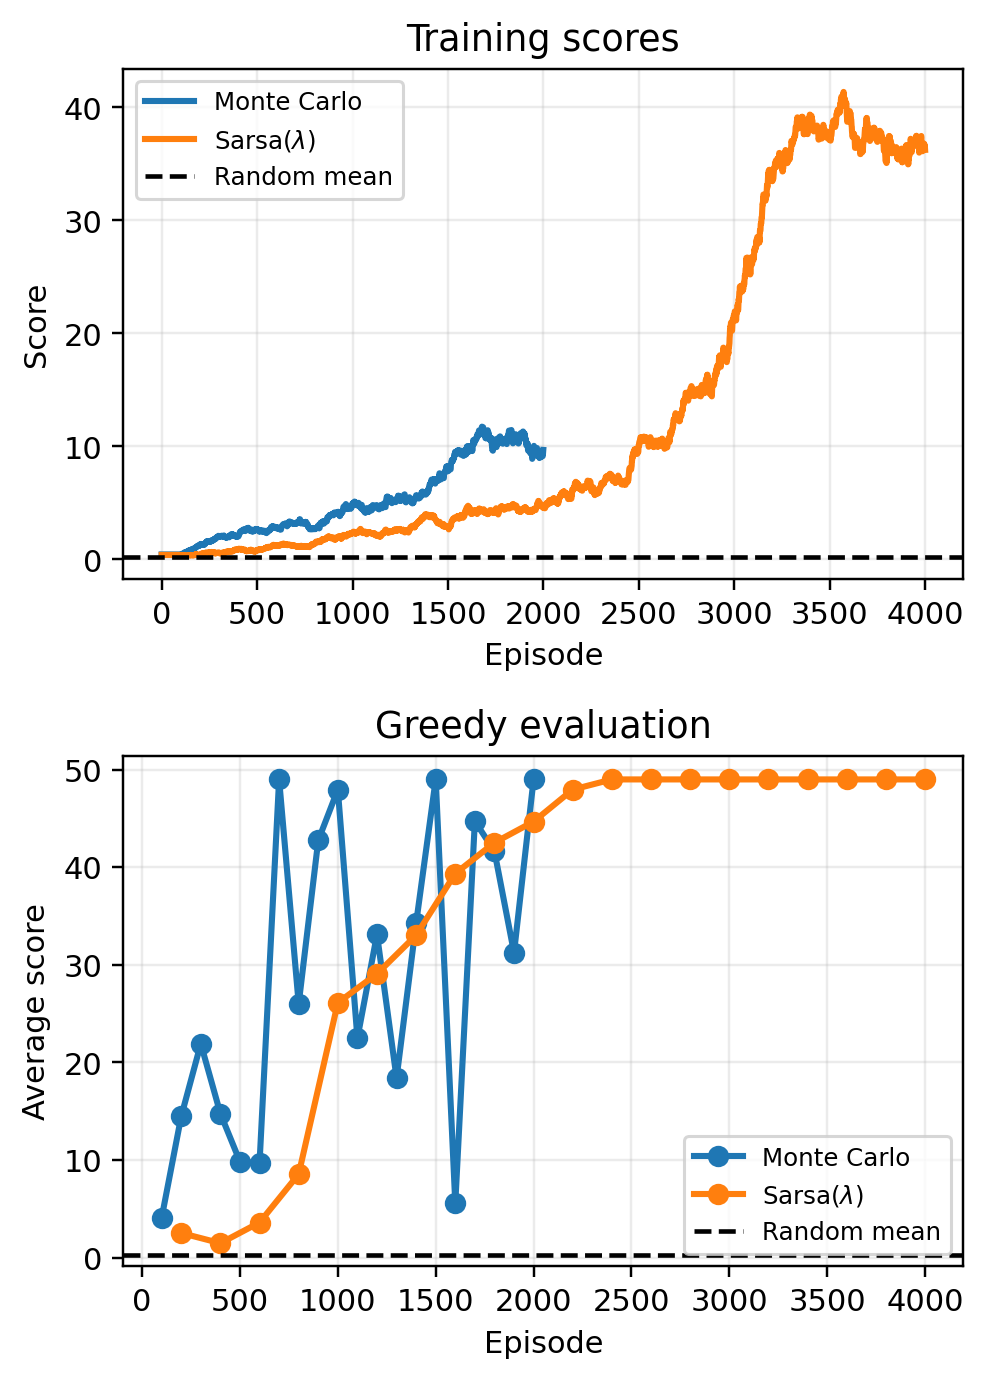
\includegraphics[width=\columnwidth]{figures/training_comparison_column.png}
\caption{Training score evolution and greedy evaluation performance. Both agents solve the environment, while Sarsa($\lambda$) reaches stronger late-training performance and a cleaner convergence profile.}
\label{fig:training}
\end{figure}

\begin{figure*}[t]
\centering
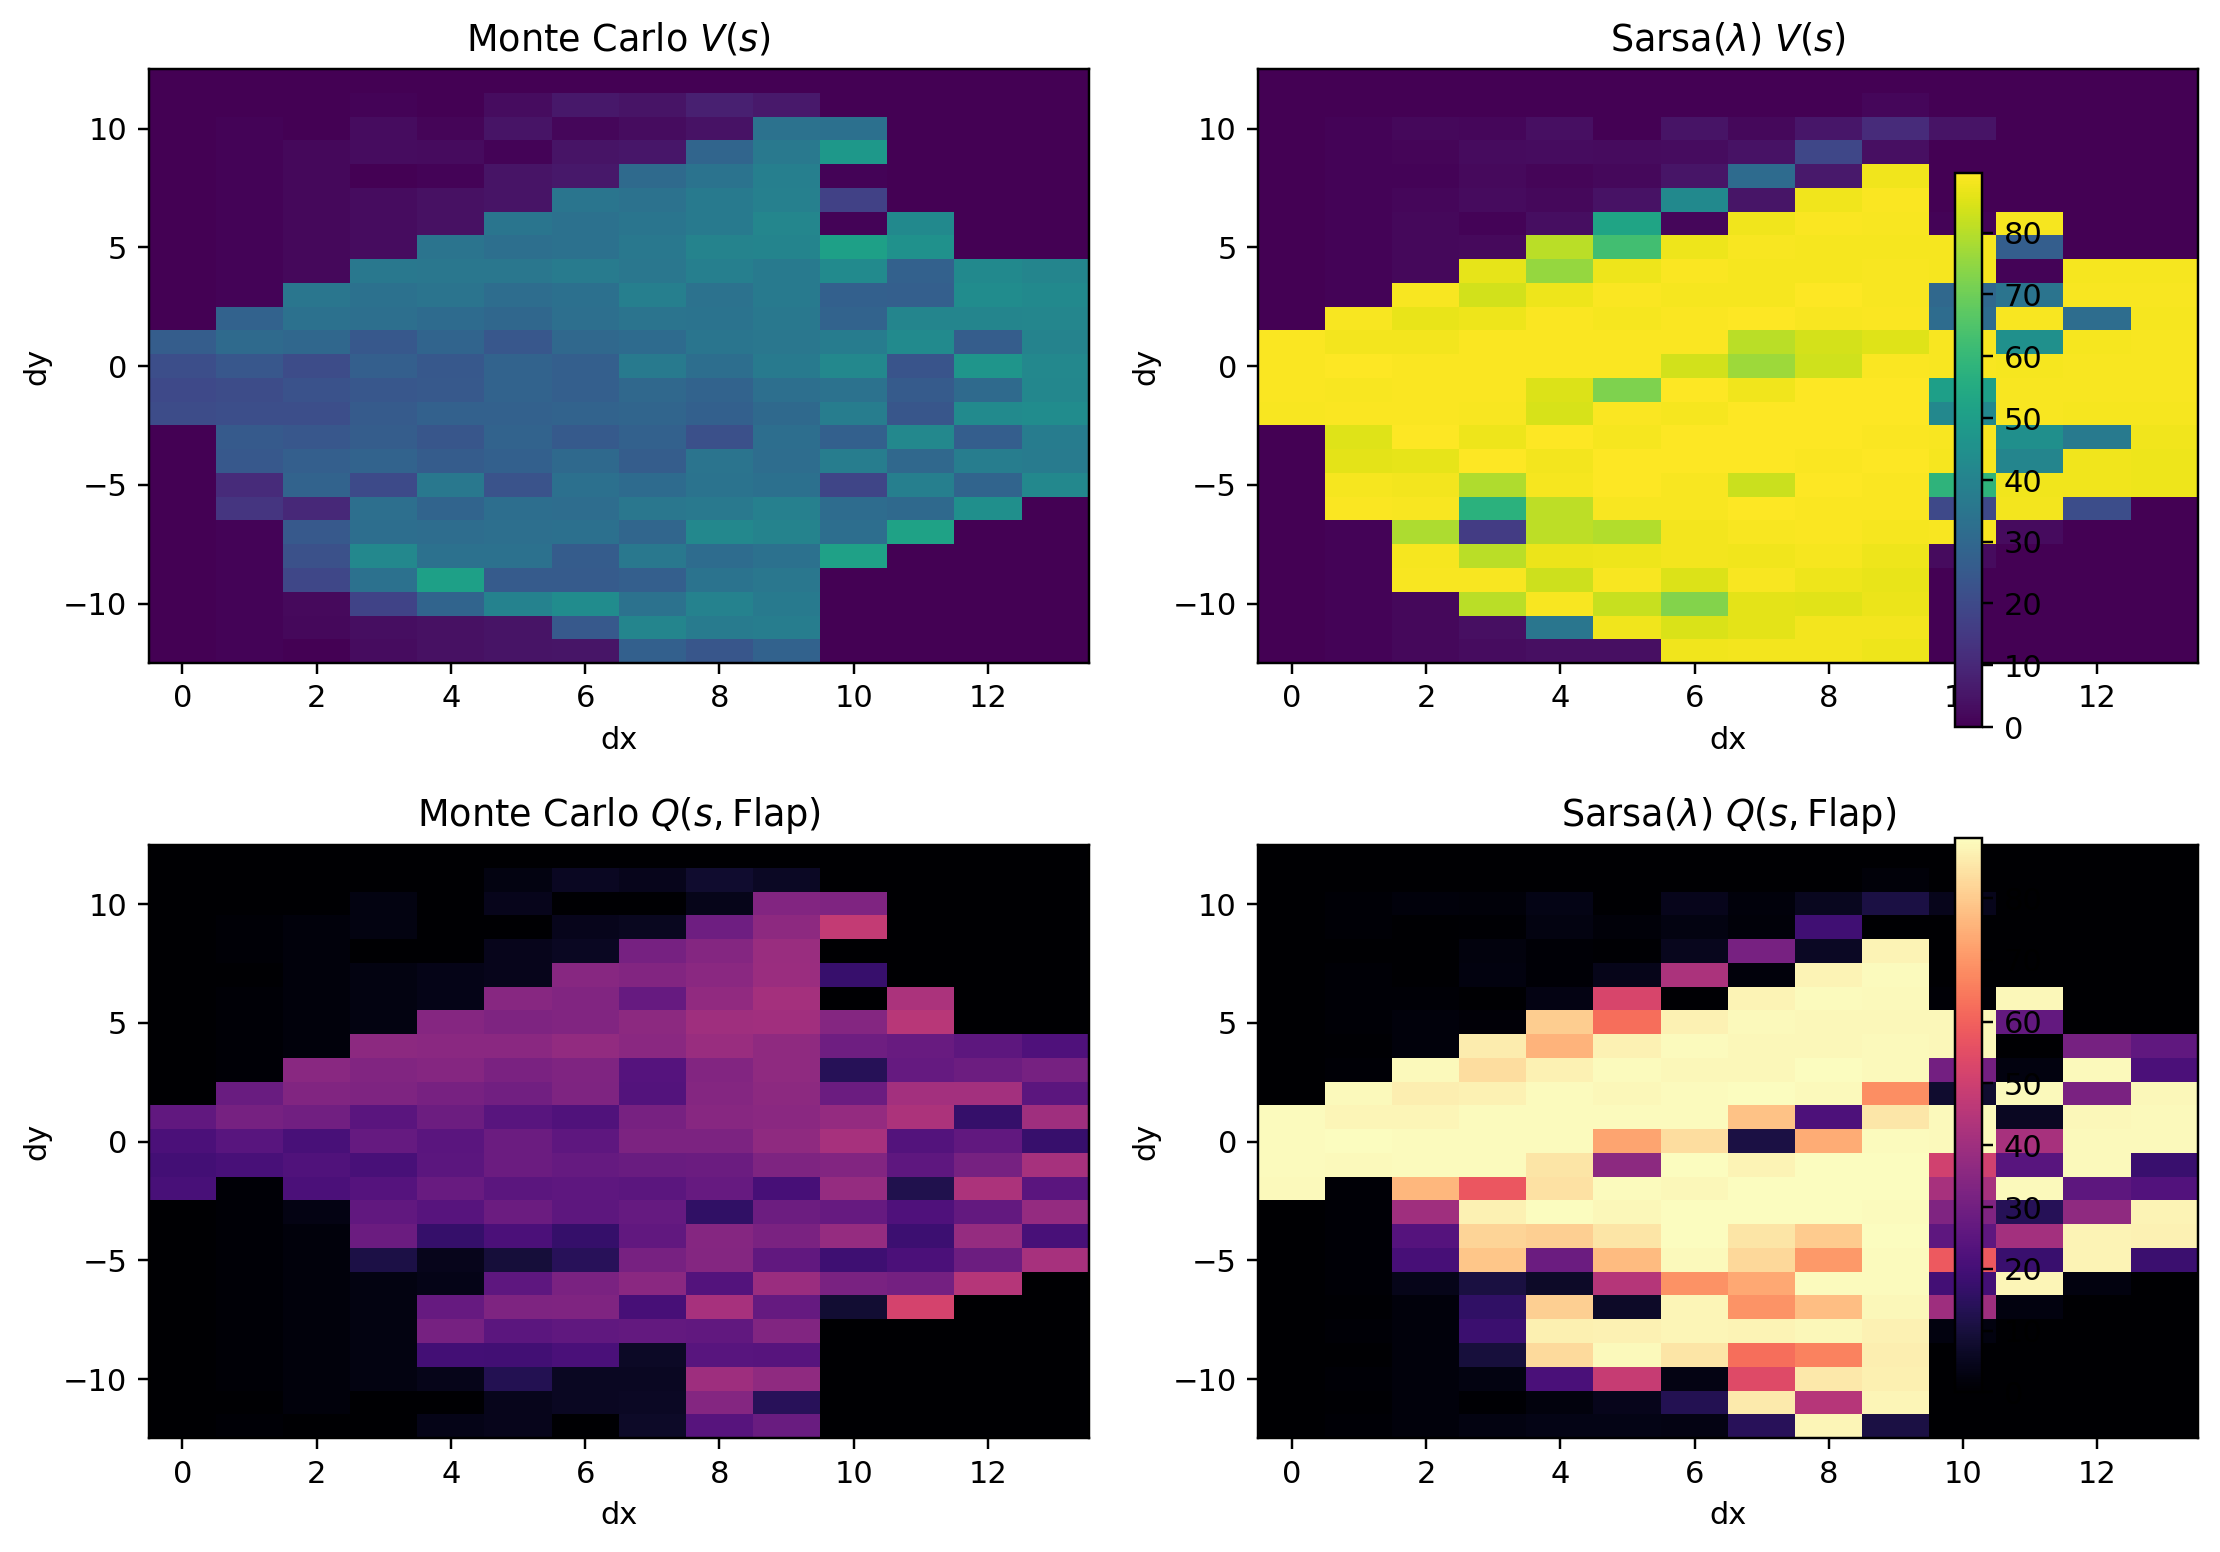
\includegraphics[width=0.96\textwidth]{figures/value_action_summary.png}
\caption{Learned state-value and action-value structure. The state-value maps $V(s)$ and the flap-specific action-value maps $Q(s,\mathrm{Flap})$ reveal a structured safe region around reachable pipe-gap states. Sarsa($\lambda$) produces smoother maps, which is consistent with its temporal-difference updates.}
\label{fig:values}
\end{figure*}

\section*{State, Action-Value Functions, and Parameter Sensitivity}
The learned value maps in Figure~\ref{fig:values} are coherent: high-value regions are concentrated around safe and reachable states rather than appearing as unstructured noise. The Monte Carlo maps are meaningful but less smooth, whereas Sarsa($\lambda$) produces more spatially regular value estimates. This matches the intuition from the learning curves.

Parameter sweeps were used to identify how robust each algorithm is to its key hyperparameters. For Monte Carlo, keeping $\varepsilon_{\text{end}}$ too large hurts final performance because the policy keeps exploring too aggressively. For Sarsa($\lambda$), the choice of $\lambda$ has a visible effect on both performance and stability. In these runs, intermediate-to-high values of $\lambda$ work best, but very large $\lambda$ also increase variance.

\section*{Environment Variants and Portability}
The two TFB versions differ only in the observation returned to the agent. \texttt{TextFlappyBird-screen-v0} returns the full game screen as an integer matrix, which is richer but much more difficult to handle with tabular reinforcement learning. \texttt{TextFlappyBird-v0} returns only $(dx,dy)$, which removes most of the representation burden and makes tabular Monte Carlo and tabular Sarsa($\lambda$) practical. The limitation of the compact version is that it is less expressive; the limitation of the screen-based version is that it is not well matched to simple tabular value tables.

The same algorithmic ideas could be transferred to the original Flappy Bird environment, but not always in exactly the same implementation. If the state is compact and low-dimensional, the same tabular methods can be reused directly. If the original environment exposes raw images, the state space becomes too large for this implementation, and function approximation or deep reinforcement learning would usually be required instead.

\section*{Generalization to a New Configuration}
To test transfer, the trained policies were evaluated on a new TFB configuration with height$=\TransferHeight$, width$=\TransferWidth$, and pipe-gap$=\TransferGap$. As expected, both agents lose performance because they were optimized for a specific geometry. Nevertheless, Sarsa($\lambda$) transfers better: its average greedy score on the new configuration is \textbf{\SarsaTransferScore{}} against \textbf{\MCTransferScore{}} for Monte Carlo, while both agents remain perfect on the training configuration (\MCTrainScore{} and \SarsaTrainScore{} respectively). This suggests that Sarsa($\lambda$) learns a policy that is not only strong in-distribution, but also more robust under moderate environment changes.

\begin{figure}[t]
\centering
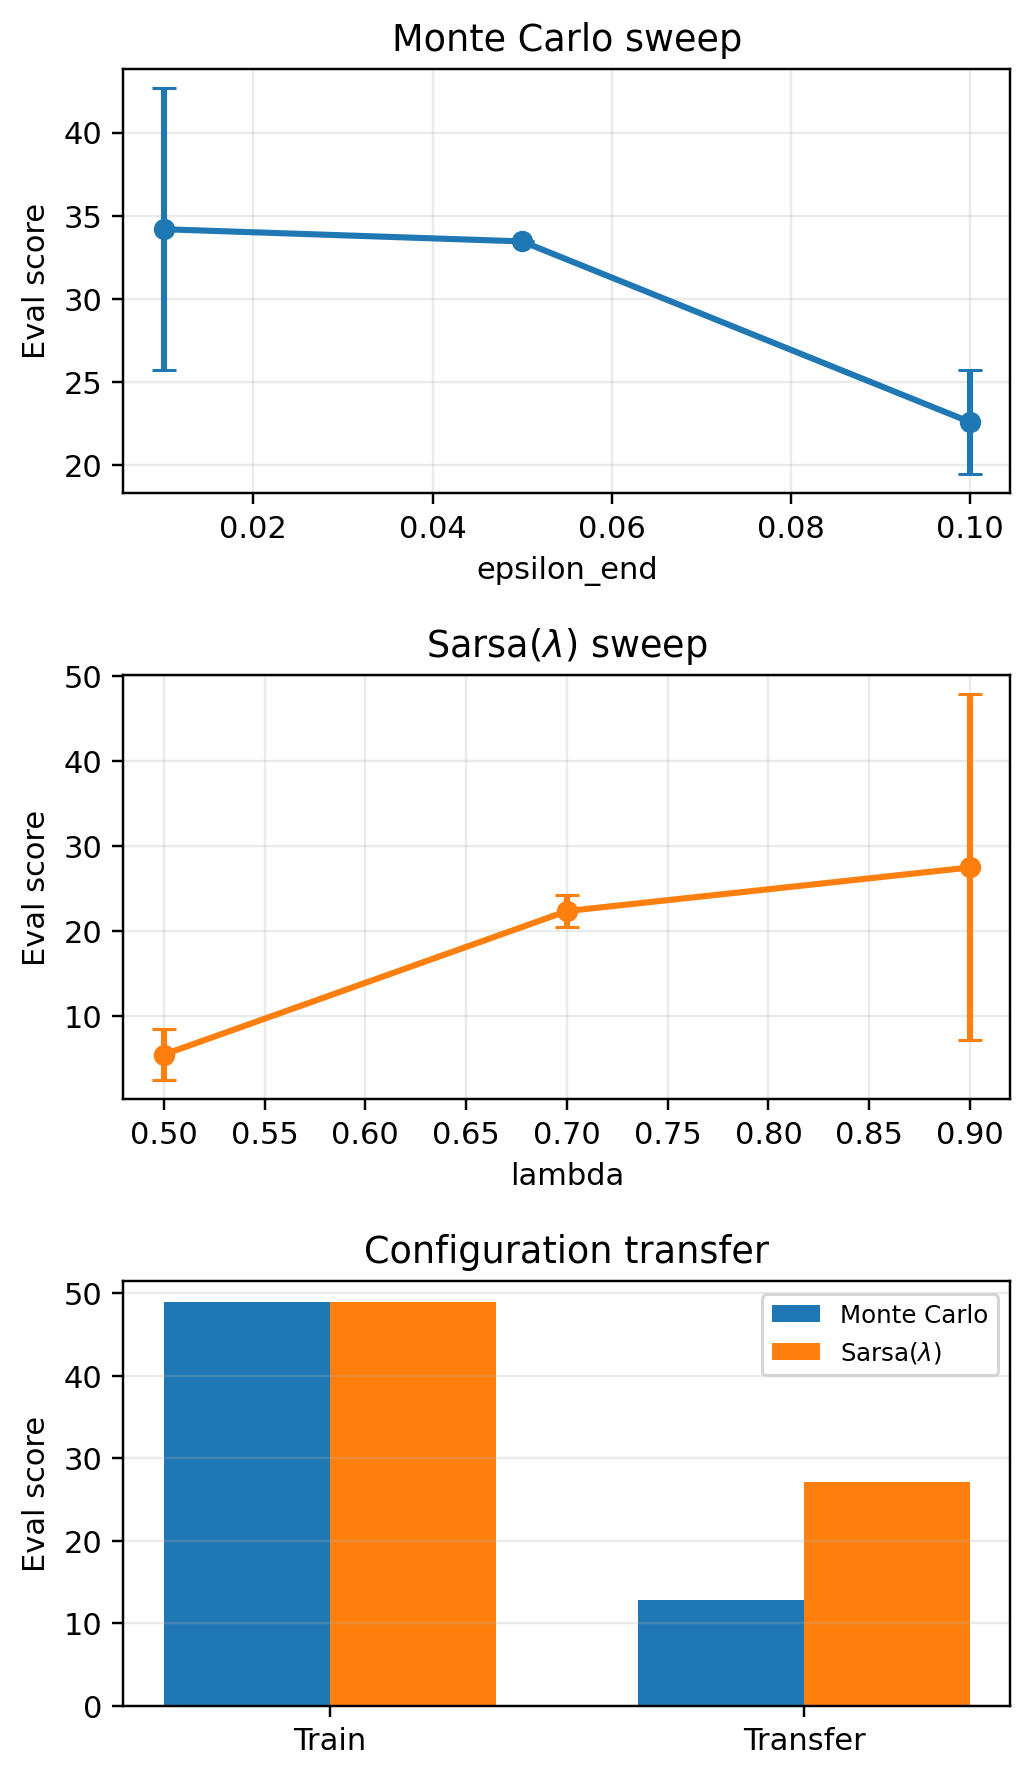
\includegraphics[width=\columnwidth]{figures/parameter_transfer_column.png}
\caption{Hyperparameter sensitivity and transfer behaviour. Monte Carlo is sensitive to residual exploration, while Sarsa($\lambda$) is sensitive to the eligibility-trace parameter and transfers better to the new level configuration.}
\label{fig:sweeps}
\end{figure}

\section*{Conclusion}
Both implementations successfully solve \texttt{TextFlappyBird-v0}. Monte Carlo control eventually reaches optimal behaviour, but Sarsa($\lambda$) learns faster, produces smoother value estimates, and generalizes better to the tested level change. Overall, the compact TFB environment is well suited to tabular reinforcement learning, while the screen-based version would likely require a stronger representation model to be competitive.

\begin{thebibliography}{9}
\bibitem{sb} Sutton, R.S., Barto, A.G.: \emph{Reinforcement Learning: An Introduction}. 2nd edn. MIT Press (2018)
\bibitem{tfb} Christodoulidis, S.: Text Flappy Bird Gym. \url{https://gitlab-research.centralesupelec.fr/stergios.christodoulidis/text-flappy-bird-gym}
\bibitem{fbgym} Talendar: Flappy Bird Gym. \url{https://github.com/Talendar/flappy-bird-gym}
\end{thebibliography}

\end{document}
